\documentclass{article}
\usepackage[compat=1.1.0]{tikz-feynman}
\begin{document}

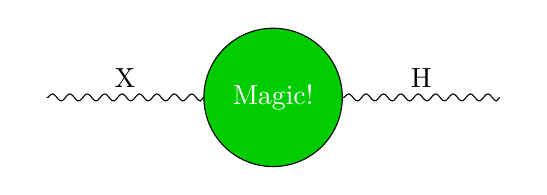
\begin{tikzpicture}
  \begin{feynman}
    \vertex (a) at (0,0) {};
    \vertex[blob,fill=black!20!green,minimum size = 50pt] (b) at (3,0) {\color{white} Magic!};
    \vertex (c) at (6,0) {};
    
    \diagram* [horizontal=a to b] {
      (a) -- [photon,edge label=X] (b) -- [photon,edge label=H] (c),
      };
    \end{feynman}
    % \node (n1) at (1,-0.05) {H};
\end{tikzpicture}

\end{document}

%%% Local Variables:
%%% mode: latex
%%% TeX-master: t
%%% End:
